
\section{Generating realistic data} %0.5-1

We as humans have been born with the blessing of intelligence. We use this intelligence to create things of indescribable creativity and complexity and it is these things that give a deeper meaning to large parts of human life. All the greater is the drive to understand this creative process and to reproduce it artificially. And it is this drive that gave rise to a completely new branch of research in computer sciences, which finally led to the concept of \textit{Generative Modeling}.

Generative Modeling is an umbrella term describing artificial approaches to generate realistic data. The current state-of-the-art approaches are dominated by so called \textit{Deep Neural Networks}, complex artificial constructs which are partially inspired by the human brain. These networks are implemented as a computer program, using modern machine learning libraries such as \textit{PyTorch} or \textit{Tensorflow}.

In the last years generative modeling has seen an \textbf{immense} progress in generating the most diverse types of data. Some results have even reached such a quality that they can hardly be distinguished from realistic data for the human eye. Some fields of generative modeling on which outstanding results have been achieved include image generation, video generation and audio and speech generation. In addition to the general push for better generation models, some models are already indispensable for various application purposes such as image processing, anomaly detection in medical context and generation of new data for scientific uses, e.g. the artificial generation of promising molecular candidates for the development of new effective drugs \cite{molgrad}.

\section{Score-Based Models - The new contenders to GANs?} %0.5-1

\section{Semantic Segmentation and Semantic Synthesis} 
%
\begin{figure}[h!]
    \centering
    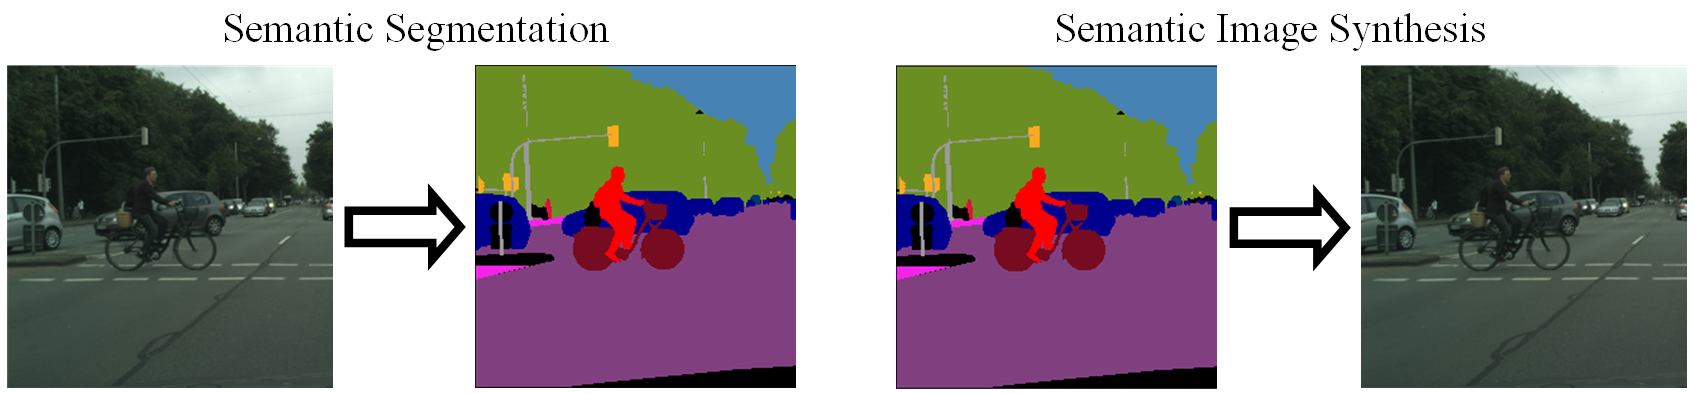
\includegraphics[width=1\textwidth]{Chapters/figures/sem_seg_vs_sem_synth.PNG}
\end{figure}
%
Two large fields in image based machine learning are semantic segmentation and semantic image synthesis. In semantic segmentation so called semantic segmentation networks have the task of a pixel-wise classification of images. In semantic image synthesis – unlike unconditioned image generation \cite{score_3} – images are generated based one a given semantic label map.

In this thesis we show that Score-Based Generative Models, with the help of semantic segmentation networks, are capable of synthesizing realistic looking images based on semantic label maps for various resolutions up to $1024\times512$ and datasets such as Cityscapes \cite{cityscapes}, ADE20K \cite{ade20k} and landscape images scraped from flickr. We show that the synthesized images for some categories can keep up with or even surpass state of the art generative models such as CRN \cite{crn}, pix2pixHD \cite{pix2pixHD}, and SPADE \cite{spade}, although there is still room for further improvement. We therefore show how the current technique could be optimized in future work to yield even better results. 

The implementation for this work is done with PyTorch and the code is publicly available on GitHub at the following links: 
\begin{itemize}
    \item https://github.com/TimK1998/SemanticSynthesisForScoreBasedModels
    \item https://github.com/TimK1998/SemanticSegmentation
\end{itemize}
